\section{Quality Control}
Data processing can be performed as non-recursive (batch least-squares) or as recursive
least-squares estimation. This section contains a brief description of the models involved
and the related procedures for testing and reliability. A typical example is the situation
of possible cycle slips in the carrier phase observation. The alternative hypotheses may
consist of cycle slips in GPS carrier observations.
	\subsection{The Non-Recursive Case}
	In hypothesis testing, one usually calls the case without any model errors the null hypoth-esis $H_0$. An alternative hypothesis $H_a$ assumes there is a bias in one or several of the
	observations. Let c be a known m-vector specifying the model error, x be the n-vector of
	unknowns and s its unknown size. Then two hypotheses are defined as
	\begin{equation}
	H_0: b=Ax+e  \qquad weight\,C=\Sigma^{-1}_b
	\end{equation}
	\begin{equation}
	H_a:b=Ax+sc+e  \qquad weight\,C=\Sigma^{-1}_b.
	\end{equation}
	We assume that $m > n$.
	
	Assuming each alternative hypothesis describes the case of a single bias in an observation, the c-vectors consist of canonical unit vectors. The solution to (4.101) under the null hypothesis is given by
	\begin{equation*}
	\begin{split}
	\hat{x}&=(A^TCA)^{-1}A^TCb\\
	\Sigma_{\hat{x}}&=(A^TCA)^{-1}
	\end{split}.
	\end{equation*}
	Testing $H_0$ against $H_a$ consists of three steps:
	
	Detection\; An overall model test determines if unspecified model errors have occurred.
	
	Identification\; If a model error is detected, its potential source is identified by testing the
	original or nominal observation model (4.101) against models extended with bias	parameters, such as (4.102). 
	
	Adaptation \; After the identification of the most likely source for the model error, the observation model is adapted to eliminate the biases in the parameter vector.
	
	The projector $P=I-(A^TCA)^{-1}A^TC$ projects vectors onto the column space of
	A as demonstrated in Section 6.6. The vector of residuals is $\hat{e}=b-A\hat{x}$.
	
	In the detection step the uniformly most powerful test statistic for testing $H_0$ against
	$H_a$ is given as 
	\begin{equation}
	T=\frac{(Pb)^TCb}{m-n}=\frac{\hat{e}^TC\hat{e}{m-n}}.
	\end{equation}
	T is the overall model test statistic. Under $H_0$ and $H_a$, T is F distributed:
	\begin{equation*}
	H_0:T~F(m-n,\infty ,0) \qquad H_a:T~F(m-n,\infty ,\lambda)
	\end{equation*}	 
	The non-centrality parameter $\delta$ is defined as
	\begin{equation}
	\delta=s^2c^TCPc.
	\end{equation}
	Once reference values are chosen for the level of confidence $\alpha_0$ (the probability of rejecting $H_0$ falsely), the detection power $\gamma_0$(the probability of rejecting $H_0$  when $H_a$ is true) and the number of degrees of freedom m — n, the non-centrality parameter $\delta$ can be computed. This is the B-method of testing which was described by Willem Baarda in 1968.
	
	The B-method assumes that an error related to the non-centrality parameter $\delta_0=\delta(\alpha_0,\gamma_0,1)$ is detected with equal probability $\alpha$ by all tests. In other words from $\delta_0=\delta(\alpha_0,\gamma_0,1)=\lambda(\alpha,\gamma_0,m=n)$, with $m-n>1$, the level of confidences $\alpha$ can be computed.
	Once $\delta_0$ is known, the size of the bias that can just be detected follows from (4.104) as
	\begin{equation}
	|s|=\sqrt{\frac{\delta_0}{c^TCPc}}.
	\end{equation}
	This is the Minimal Detectable Bias (MDB). As can be seen from (4.105), the MDB depends on $\alpha_0,\gamma_0$, and the functional and stochastic model, through the design matrix A and
	the covariance matrix $\Sigma_b$ and the alternative hypothesis captured in the vector c.
	
	Remark 4.4\; We bring a detailed description of a procedure for computation of the non-centrality parameter $\delta$.
	
	First the central case (null hypothesis $H_0$): select a value for a which is the probability of an error of the first kind, that is rejecting $H_0$ falsely.
	
	MATLAB uses left tail and we need right tail, so we define $p=1-\alpha$. The number
	of degrees of freedom is f = m - n. The critical value is computed as x = chi2inv(p,f).
	This is the value where the critical region starts (rejection of $H_0$) and extends to $+\infty$.
	
	Next the non-central case (alternative hypothesis $H_a$): We know the critical value x
	and the number of degrees of freedom f, and must solve p = ncx2cdf (x,f,delta ) iteratively
	such that $\delta$ yields the known value for p.
	
	The solution from this iteration yields $\beta=p$(left tail probability of accepting $H_0$,
	while $H_0$ is true). The probability of correct decision is the “power” $\gamma=1-\beta$.
	
	For most GPS applications we set $\alpha_0=0.001,\gamma_0=0.80$ (or even higher) resulting
	in a non-centrality parameter of $\delta_0\approx 17$, see Figure 4.13. The computation is done by the M-file cct.
	
	\begin{figure}[h]
		\centering
		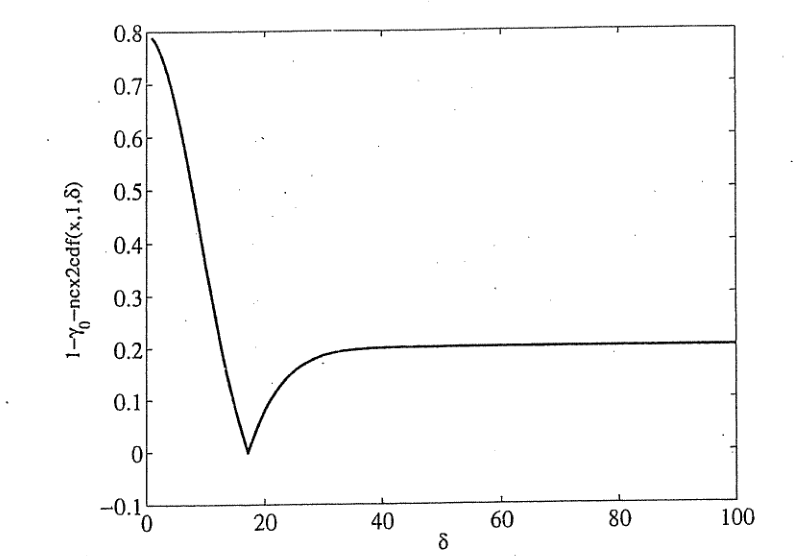
\includegraphics[width=0.7\linewidth]{TeX_files/Part02/chapter04/image/4-13}
		\caption{Figure 4.13\; The function $1-\gamma_0-ncx2cdf(x,1,\delta)$ as function of $\delta$}
		\label{fig:4-13}
	\end{figure}
	
	If the test statistic T exceeds a threshold, we say we have detected a bias s and
	the sources of the possible errors have to be found in the identification step. In practice
	this is accomplished by testing a number of alternative hypotheses, each describing one
	model error at a time, see (4.102). The uniformly most powerful test statistic for testing
	$H_0$ against $H_a$ is given as
	\begin{equation}
	t=\frac{(Pc)^TCPb}{\sqrt{(Pc)^TCPc}}=\frac{c^TCPb}{\sqrt{c^TCPc}}.
	\end{equation}
	This expression is known as a slippage test statistic. Under $H_0$ and $H_a$ the slippage test
	statistic is normally distributed
	\begin{equation*}
	\begin{split}
	 &H_0:t~N(0,1)   \\
	 &H_a:t~N(\sqrt{(Pc)^TCPc}s,1).
	\end{split}
	\end{equation*}
	The practical procedure for identifying model errors is to determine the largest slippage test statistic (in absolute value) and perform another least-squares adjustment until the
	test statistic T is accepted, or until there is no redundancy left, i.e., until m - n = 0 . Once the largest slippage test statistic t has been found, its likelihood needs to be tested. The	likelihood of the identified model error can be tested by comparing the test statistic with the critical value $N_{\alpha_0/2}(0,1)$ where $\alpha_0$ is the level of confidence. If the largest slippage test statistic t in each cycle exceeds the critical value, i.e, if
	\begin{equation*}
	|t|>N_{\alpha_0/2}(0,1)
	\end{equation*}
	then it is likely that a model error has been identified. If not, one should extend the set of alternative hypotheses to consider.
	
	For the adaptation step, several alternatives exist. One way to adapt would be to
	simply discard the bad observations (as already done, actually, in the iterated identification
	step), another to extend the vector of unknowns by one or more additional parameters.
	
	The alternative hypotheses may consist of outliers and cycle slips in GPS code and
	carrier observations, respectively. The MDB is said to describe the internal reliability of
	a system. External reliability is defined as the influence of a bias s with size equal to the
	MDB on the estimated parameters sx:
	\begin{equation*}
	sx=(A^TCA)^{-1}A^TCcs=\Sigma_{\hat{x}}A^TCcs.
	\end{equation*} 
	It should be noted that to compute internal and external reliability parameters, no actual
	data is required. They can already be computed in the design or planning phase of a survey.
	
	\subsection{The Recursive Case}
	The main difference with non-recursive or batch least squares is that for recursive least
	squares the unknown parameters are updated whenever new observations become available. Assuming the unknown parameters remain the same for an entire observation period,
	the null and alternative hypothesis for an epoch k are defined as 
	\begin{equation*}
	\begin{split}
	&H_0:b_k=A_kx   \\
	&H_a:b_k=A_kx +s_kc.
	\end{split}
	\end{equation*}
	Here we assume that a bias $s_k$ is detected and identified at the same epoch it occurred.
	in other words, we consider only local alternative hypotheses as opposed to global ones,
	which consider a number of (or even all) epochs before detecting and identifying the bias.
	Assuming a solution $\hat{x}_{k|k-1}$ with covariance matrix $P_{k|k-1}$ is available (where the subscript (k - 1) means that all epochs up to and including k - 1 were used to compute
	this solution), the recursive solution for k epochs of data under the null hypothesis is given
	as
	\begin{equation*}
	\hat{x}_{k|k}=\hat{x}_{k|k-1}+K_k(b_k-A_k\hat{x}_{k|k-1}) 
	\quad and \quad
	P_{k|k}=(I-K_kA_k)P_{k|k-1}
	\end{equation*}
	with
	\begin{equation*}
	K_k=P_{k|k-1}A^T_k(A_kP_{k|k-1}A^T_k+\Sigma_{e,k})^{-1}.
	\end{equation*}
	The vector
	\begin{equation}
	i-k=b_k-A_k\hat{x}_{k|k-1}
	\end{equation}
	is known as the innovation. Its covariance matrix is
	\begin{equation}
	\Sigma_i=A_kP_{k|k-1}A^T_k+\Sigma_{e,k}.
	\end{equation}
	Alternatively, the matrices $K_k$ and $P_{k|k}$ may be written as
	\begin{equation*}
	\begin{split}
	K_k &= P_{k|k}A^T_k\Sigma^{-1}_{e,k}\\
	P_{k|k} &=(P^{-1}_{k|k-1}+A^T_k\Sigma^{-1}_{e,k}A_k)^{-1}.
	\end{split}
	\end{equation*}
	Let $m_k$ be the number of observations at epoch k. For the detection and identification step,
	the local overall model test statistics T and local slippage test statistics t are given by
	\begin{equation*}
	\begin{split}
	&T=\frac{i^T_k\Sigma^{-1}_ii_k}{m_k}\\
	&t=\frac{c^T\Sigma^{-1}_ii_k}{\sqrt{c^T\Sigma^{-1}_ic}}
	\end{split}
	\end{equation*}
	which under $H_0$ and $H_a$ are distributed as
	\begin{equation*}
	H_0:T~F(m_k,\infty ,0) \qquad H_a:T~F(m_k,\infty ,\delta)
	\end{equation*}	
	and
	\begin{equation*}
	H_0:t~N(0,1) \qquad H_a:t~N(\sqrt{c^T\Sigma^{-1}_ic}s,1).
	\end{equation*}
	The expression for the MDB reads
	\begin{equation*}
	|s|=\sqrt{\frac{\delta_0}{c^T\Sigma^{-1}_ic}}.
	\end{equation*}
	The influence of a bias with size equal to the MDB on the estimated parameters is given as
	\begin{equation*}
	sx=sK_kc.
	\end{equation*}
	For further reading, see Teunissen \& Kleusberg (1998), Chapter 7 on “Quality Control and GPS .”
	

1\; For two independent measurements $x= b_1$ and $x= b_2$, the best $\hat{x}$ should be some
weighted average $\hat{x}=ab_1+(1-a)b_2$. When $b_1$ and $b_2$ have mean zero and
variances $\sigma^2_1$ and $\sigma^2_2$, the variance of $\hat{x}$ will be $P=a^2\sigma^2_1+(1-a)^2\sigma^2_2$. Choose the number a that minimizes P: dP/da = 0.

Show that this a gives the weighting which we have claimed to be best, using weights
$w_1=1/\sigma_1$ and $w_2=1/\sigma_2$.

2\; After N = 4 coin flips (binomial distribution) what are the five probabilities $p_0,p_1,...,p_4$ of M = 0,1,..., 4 heads? Find the mean $\bar{M}=\Sigma Mp_M$.
Show that the variance $\sigma^2=\Sigma(M-\bar{M})^2 p_M$ agrees with N/4 = 1.

3\; (a) At the center of Figure 4.3 with N = 4 and $\sigma^2=N/4 = 1$, check that the actual
height $p_2=\frac{6}{16}$ is a little below the Gaussian $p(x)=1/\sqrt{2\pi}\sigma$.

(b) The center of the Gaussian with $\sigma=\sqrt{N}/2$ has height $\sqrt{2\pi N}$. Using Stirling's approximation to N! and (N/2)!, show that the middle binomial coefficient $p_{N/2}$
approaches that height: 	
\begin{equation*}
(M=\frac{N}{2})   \quad p_{N/2}=\frac{N!}{((N/2)!)^2}\approx \frac{(N/e)^N\sqrt{2\pi N}}{((n/2e)^{N/2}\sqrt{\pi N})^2}=?
\end{equation*}	

4\; The variance $\sigma^2=\Sigma(n-\bar{n})^2p_n$  is computed around the mean $\bar{n}=\Sigma np_n$. Expand $(n-\bar{n})^2=n^2-2n\bar{n}+\bar{n}^2$ to show that this $\sigma^2$ equals $(\Sigma n^2p_n)-\bar{n}^2$.

5\; Imagine a line of masses $p_0,...,p_n$ at the points x = 0,...,n. Explain how the
mean $E\{x\}$ with probabilities $p_j$ corresponds to the center of mass. The variance $\sigma^2$
is the moment of inertia around what point?

6\; Start with r independent random variables $X_1,...,X_r$ with variances $\sigma^2_1,...,\sigma^2_r$. Show that the sum $X=X_1+...+X_r$ has variance $\sigma^2_1+...+\sigma^2_r$.

7\; One flip of a weighted coin has M = 1 (heads) with probability p and M = 0 (tails)
with probability q = 1 - p. What are the mean $\bar{M}$ and the variance $\sigma$? What are
the mean and variance for the number M of heads after N coin flips?

8\; Suppose every number is rounded down to the nearest integer. The distribution of
rounding errors e is still uniform, but on what interval of e's? What is the mean m?
What is the variance around the mean $\int(e-m)^2$ de?

9\; Suppose the random variable X has mean $\mu$ and variance $\sigma^2$.

(a) \; Show that the new variable Y = aX + b has mean $a\mu+b$.

(b) \; Show that the variance of Y is $a^2\mu^2$.

10\; Suppose X is a vector of random variables, each with mean zero, and Y = LX is
related to X by a fixed matrix L(m by n). Derive from (4.16) the “Law of Covariance
Propagation” which brings L and $L^T$ outside:
\begin{equation*}
\Sigma_Y=L\Sigma_XL^T \quad or \quad E\{YY^T\}=LE\{XX^T\}L^T.
\end{equation*}
Problems 11-14 give experience with a small-size Kalman filter

11\; In Example 4.6, extend the matrix A to 5 by 3 with $x_3-x_2=c_2$ and a new measurement
$x_3=b_3$. With unit variances in C = I, solve $A^TA\hat{x}=A^Tb$ for the best estimates $\hat{x_1},\hat{x_2},\hat{x_3}$.

Solution: With $c_1=c_2=0,\hat{x}_{3|3}=\frac{1}{8}(b_1+2b_2+5b_3)$ and $P_{3|3}=\frac{5}{8}$.

12\; In Problem 11, continue the Kalman recursion from $\hat{x_{2|2}}$ in the text to predict 
$\hat{x_{3|2}}$ and correct to $\hat{x_{3|3}}$. As in Example 4.7, find their variances $P_{3|2}$ and $P_{3|3}$ from the last entries in $(A^TA)^{-1}_{3|2}$ and $(A^TA)^{-1}$.

13\; In this Kalman example, the determinants of $A^TA$ come from the Fibonacci numbers
1,1,2,3,5,8,... as new rows are added to A. Find the three pivots of $(A^TA)_{3|3}$ as
ratios of Fibonacci numbers:
\begin{equation*}
A^TA=
\begin{bmatrix}
2&-1&0\\
-1&3&-1\\
0&-1&2
\end{bmatrix}
LDL^T  \quad with\,pivots\,in\,D.
\end{equation*} 	
14\; For $\sigma^2_1=\sigma^2_2=1$ and any $v^2_1$ in (4.31), the covariance matrix is $\Sigma=diag(1,v^2_1,1)$. Solve $A^T\Sigma^{-1}A\hat{x}=A^T\Sigma^{-1}b$. What are the limiting values of $\hat{x}_i$,as $v_1\rightarrow 0$?	